\chapter{Introduction}
\label{chap:intro}

The Muon g-2 experiment E989 at Fermilab~\cite{Grange2015} aims to measure
the anomalous dipole magnetic moment $a_{\mu}$ of the muon
to a relative precision of 140\,ppb.  This would represent a fourfold improvement compared to the previous measurement~\cite{Bennett2006} at Brookhaven National Laboratory (BNL), which is more than 3 standard deviations greater than typical Standard Model (SM) predictions~\cite{Davier2010,Hagiwara2011}.  While suggestive of new physics, the situation is inconclusive and begs to be resolved.  To this end, an active theoretical and experimental campaign is in progress to reduce the uncertainties in the SM predictions and in the measurement of the anomaly.

\begin{figure}[htbp]
\centering
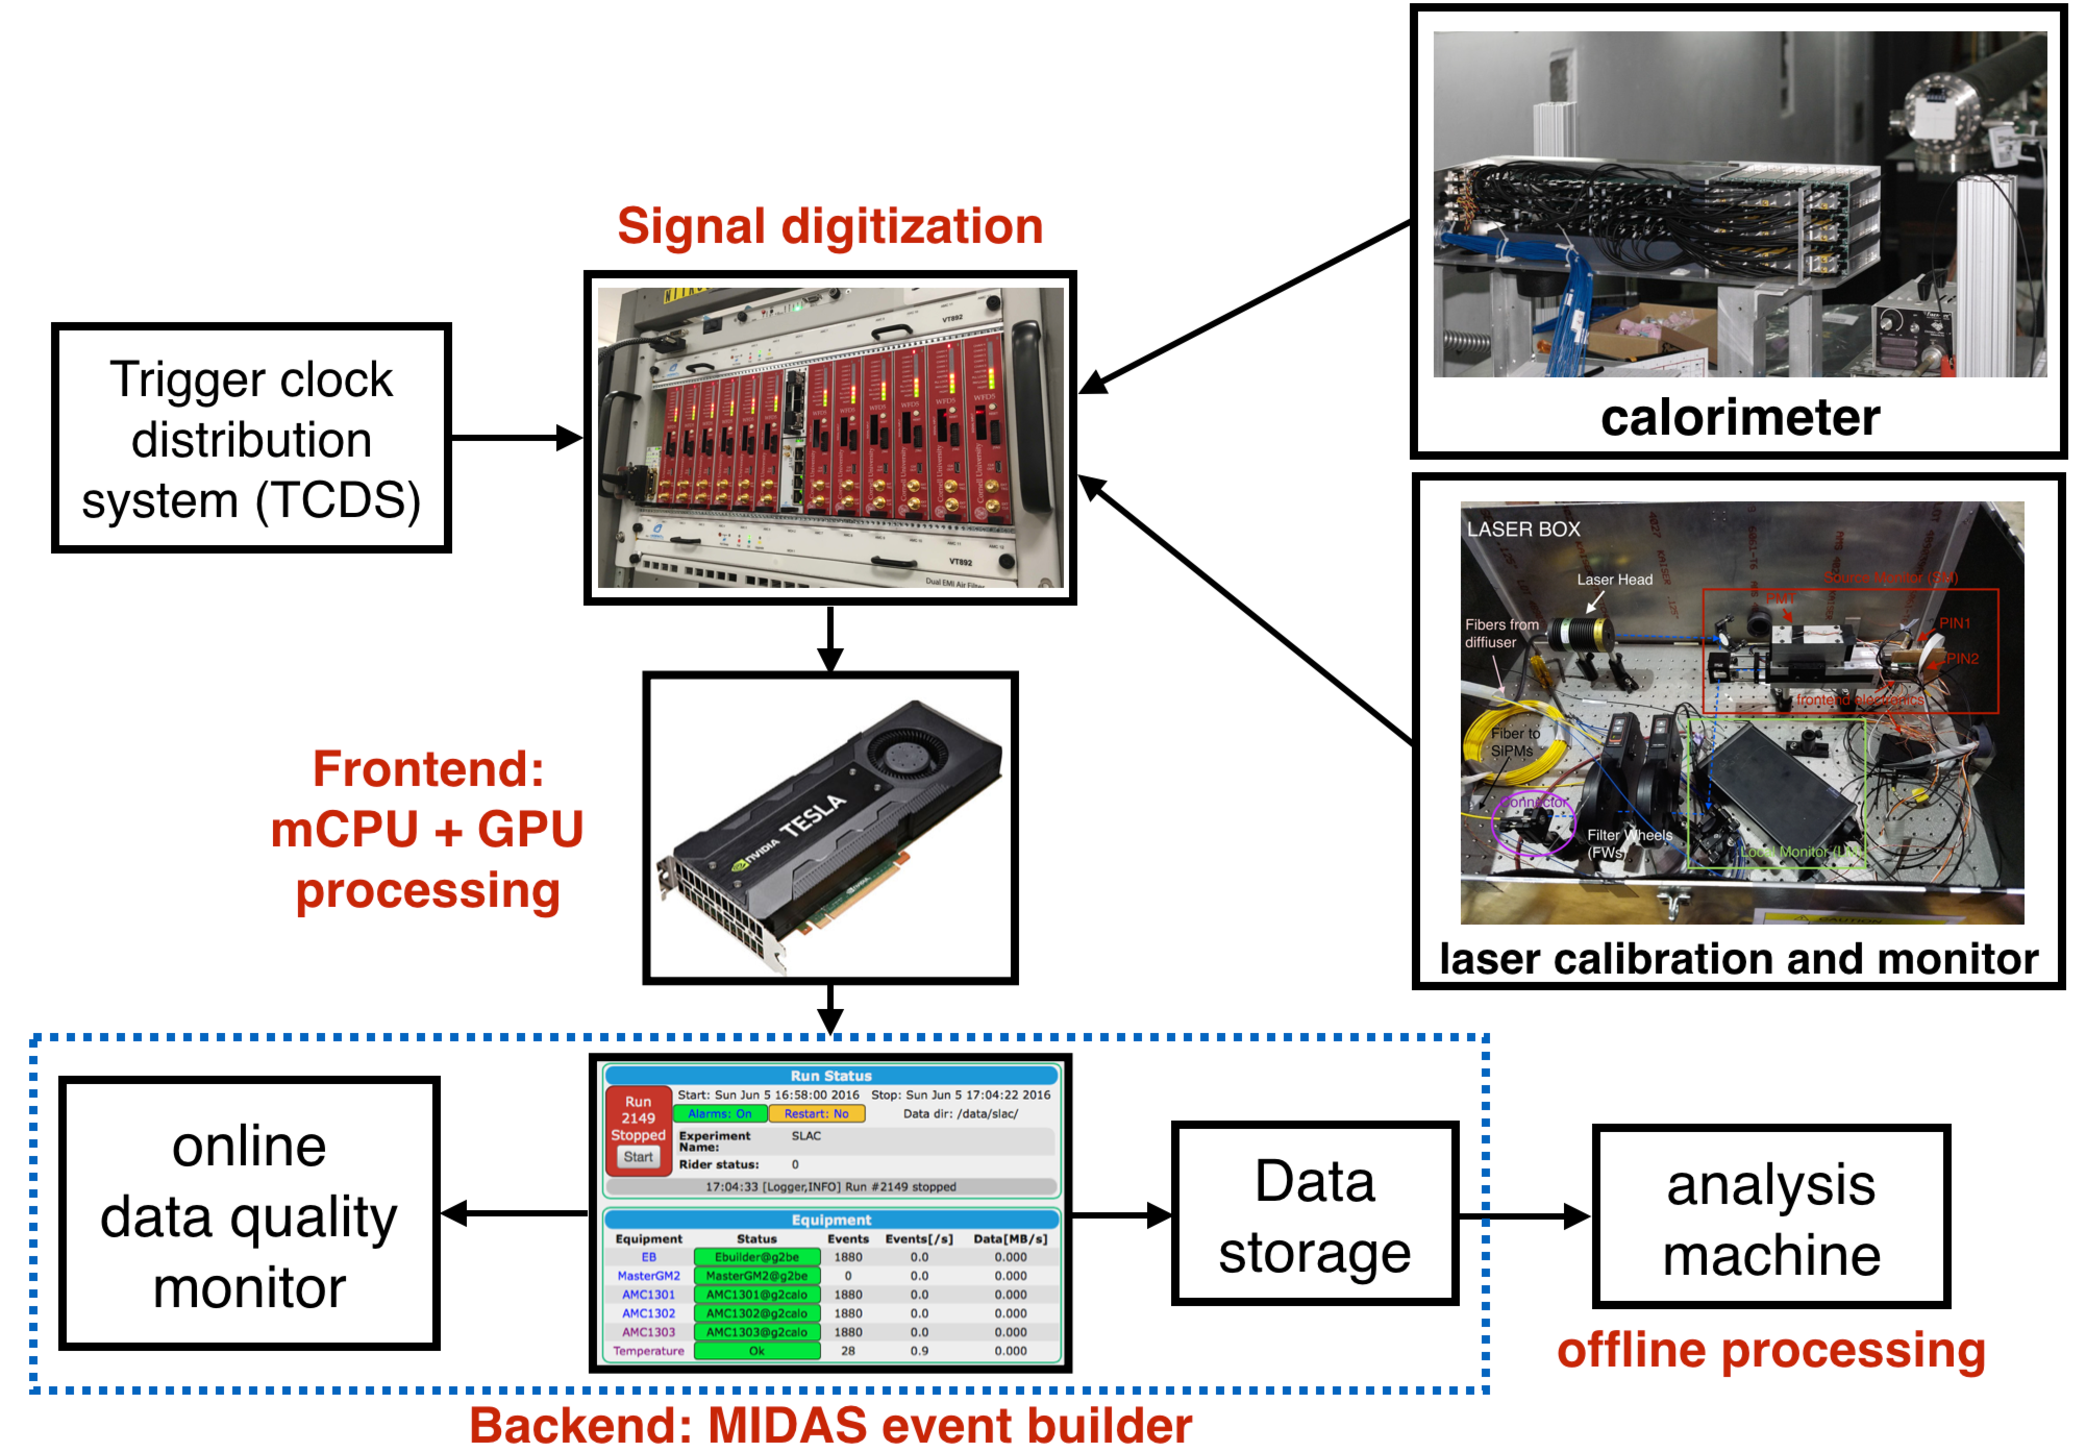
\includegraphics[width=0.95\textwidth]{pics/FullCaloSystem.pdf}
\caption{End-to-end calorimeter system for the Muon g-2 experiment at Fermilab.}
\label{fig:endtoendsystem}
\end{figure}

The E989 experiment --- which largely follows the measuring strategy of the BNL muon storage ring $a_{\mu}$ experiment --- is designed to decisively confirm or refute the finding.  The plan~\cite{Grange2015} is to collect a 21 times larger data set using a newly developed, high-purity and high-intensity polarized muon beam at Fermilab. Bunches of positive 3.1~GeV/$c$ muons will be injected into the relocated BNL superconducting storage ring at an average fill rate of 12\,s$^{-1}$.  All new measuring instrumentation as shown in Fig.~\ref{fig:endtoendsystem} is being developed to handle the much larger data set and to greatly reduce known systematic uncertainties.

A series of test beams were performed at SLAC in order to optimize the design of sub-systems. This document is mainly for the final test beam carried out in the summer 2016.

Prerequisites for the data analysis for SLAC test beam 2016 are a basic understanding of what the Muon g-2 experiment and PbF$_2$ calorimeters~\cite{Fienberg2015, Jarek2017} are, some knowledge about the electromagnetic (EM) shower and the ROOT data analysis framework~\cite{ROOT}. You can follow the exercise sheet step by step which guides you to the data analysis using the reconstructed electron EM shower clusters. Some analyses may require the use of reconstructed crystal hit, which is the basic object of forming a cluster. Advanced users are encouraged to use the FNAL's \textit{art} framework for the data analysis.
%
%trim left bottom right top
\begin{figure}[htbp]
\centering
%\fbox{\includegraphics[trim=0cm 5.5cm 0cm 5.5cm ,width=0.9\textwidth]{pics/EMShower}} guide line for trimming
\includegraphics[trim=3cm 1cm 3cm 0cm, width=0.4\textwidth]{pics/EMShower.pdf}
\caption{Illustration of the electromagnetic shower of an electron injected from the left to the right, in a $9\times6$ array PbF$_2$ calorimeter. Cherenkov lights created by the charged shower particles are collected by the Silicon Photomultipliers (SiPMs) glued to the end of the PbF$_2$ crystals.}
\end{figure}

Data analysis of this test beam has several components that are common with the Muon g-2 experiment data analysis framework~\cite{Khaw2016}. The physics objects that will be used for most of the analyses are the crystal hits and the hit clusters.
These objects are reconstructed from the digitized waveform, after going through steps like pulsing fitting, energy calibration, gain correction, time correction and hit clustering. During the first week of the test beam, all these reconstruction steps
will be refined based on the data taken and these will be taken care of by those who are familiar with the \textit{art} framework. The main focus of this documentation is on the physics analysis using high level physics objects like the crystal hit and the cluster, using a C++/ROOT standalone framework. The user can proceed to more sophisticated analysis once he/she is familiar with the tools. The standalone framework can also be used as a stepping stone to develop analysis algorithm before migrating it to the \textit{art} framework.

Several studies that will be covered for the data analysis (non-exhaustive list) are
\begin{itemize}
\item energy resolution of the calorimeter
\item position and angular resolution of the calorimeter
\item degeneracy of the position and angular information of the calorimeter
\item stability of gain monitoring system
\item pile up separation for multi-electron events
\end{itemize}

%% For myself
%% Explain the offline data analysis flow here

